%%%%%%%%%%%%%%%%%%%%%%%%%%%%%%%%%%%%%%%%
%% MCM/ICM LaTeX Template %%
%% 2022 MCM/ICM           %%
%%%%%%%%%%%%%%%%%%%%%%%%%%%%%%%%%%%%%%%%
\documentclass[12pt]{article}
\usepackage{geometry}
\geometry{left=1in,right=1in,top=1in,bottom=1in}

%%%%%%%%%%%%%%%%%%%%%%%%%%%%%%%%%%%%%%%%
% Replace ABCDEF in the next line with your chosen problem
% and replace 1111111 with your Team Control Number
\newcommand{\Problem}{A}
\newcommand{\Team}{代码附录---mby}
%%%%%%%%%%%%%%%%%%%%%%%%%%%%%%%%%%%%%%%%

\usepackage{newtxtext}
\usepackage{amsmath,amssymb,amsthm}
\usepackage{newtxmath} % must come after amsXXX

\usepackage{ctex}    %调用中文宏包
\usepackage{cite}
\usepackage{graphicx}%图片头文件
\usepackage{xcolor}
\usepackage{fancyhdr}
\usepackage{float}
\usepackage{booktabs}
\usepackage{lastpage}
\usepackage{multirow}
\usepackage{caption}
\usepackage{xcolor}
\usepackage{diagbox}
\usepackage{listings}
\usepackage{fontspec}
\usepackage{verbatim}
\usepackage{float} %指定图片位置
%\usepackage{subfigure}%并排子图 共享标题 有子标题
\usepackage{subcaption}
\usepackage{makecell}
%\usepackage{indentfirst}
\lhead{数字系统实验2 \Team}
\rhead{}
\cfoot{}

\newtheorem{theorem}{Theorem}
\newtheorem{corollary}[theorem]{Corollary}
\newtheorem{lemma}[theorem]{Lemma}
\newtheorem{definition}{Definition}

\begin{document}
\graphicspath{{images}}  % Place your graphic files in the same directory as your main document
\DeclareGraphicsExtensions{.pdf, .jpg, .tif, .png, .webp}
\thispagestyle{empty}
\vspace*{-16ex}
%\centerline{\begin{tabular}{*3{c}}

%%%%%%%%%%% Begin Summary %%%%%%%%%%%
% Enter your summary here replacing the (red) text
% Replace the text from here ...
%\begin{center}
    \section*{Summary}
\end{center}



\section*{Keywords} %%%小写

% to here
%%%%%%%%%%% End Summary %%%%%%%%%%%
\setlength{\headheight}{15pt}
%\clearpage
%%%%%%%%%%%%%%%%设置目录%%%%%%%%%%%%%%
\pagestyle{fancy}
% Uncomment the next line to generate a Table of Contents
%\tableofcontents 
%\tableofcontents
\setcounter{page}{1}
\rhead{Page \thepage\ of \pageref{LastPage}}
%%%%%%%%%%%%%%%%%%%%%%%%%%%%%%

%%%%%%%%%%%%%%%%开始正文%%%%%%%%%%%%%%
%\newpage
%\section{设计名称}
去除干扰蜂鸣音
%\section{实验目的}
\begin{table}[!ht]
    \centering
    \begin{tabular}{|l|}
    \hline
        电梯处于1楼,按KEY3,LED3亮,电梯处于上行状态,楼层显示1;运行5秒至2楼后LED3灭,2楼待机。 \\ \hline
        电梯处于2楼,按KEY2,LED2亮,电梯处于下行状态,楼层显示2;运行5秒至1楼后LED2灭,1楼待机。 \\ \hline
        电梯处于1楼,按KEY1,LED1亮,电梯处于上行状态,楼层显示1;电梯运行至2楼后LED1灭,2楼待机。 \\ \hline
        电梯处于2楼,按KEY0,LED0亮,电梯处于下行状态,楼层显示2;运行至1楼后LED0灭,1楼待机。 \\ \hline
        电梯处于1楼,按KEY0或KEY2,指示灯均不应该亮,电梯1楼待机。 \\ \hline
        电梯处于1楼,按KEY3,LED3亮,电梯处于上行状态时,立刻按 KEY2,LED2亮,电梯继续运行至2楼,LED3灭;然后电梯自动返回1楼待机,LED2灭。 \\ \hline
        电梯处于1楼;按KEY3,LED3亮,电梯处于上行状态时,立刻按 KEY0,LED0亮,电梯继续运行至2楼,LED3灭;然后电梯自动返回1楼待机,LED0灭。 \\ \hline
        电梯处于1楼,按KEY1或 KEY3,让电梯运行至2楼待机;再按KEY1/ KEY3,指示灯均不应该亮,电梯继续待机。 \\ \hline
        电梯处于2楼,按KEY2,LED2亮,电梯处于下行状态时,立刻按 KEY3,LED3亮,电梯继续运行至1楼,LED2灭;然后电梯自动返回2楼待机,LED3灭。 \\ \hline
        电梯处于2楼,按KEY2,LED2亮,电梯处于下行状态时,立刻按 KEY1,LED1亮,电梯继续运行至1楼,LED2灭;然后电梯自动返回2楼待机,LED1灭。 \\ \hline
        将复位开关SW11拨至下方,电梯运行至1楼(运行时间5S)。 \\ \hline
        将启动开关SW0拨至下方,按任意按键均无反应。 \\ \hline
    \end{tabular}
\end{table}

%\section{设计要求}
\indent 提供一个包含某人说话语音片段的声音文件( buzz.wav ),但该语音信号被一个包含有几个谐波分量的蜂鸣信号干扰了。
\begin{itemize}
    \item [\textbf{1.}] 用Matlab的wavread命令读取该声音文件。注意,该命令可以同时得到声音文件的采样率和采样位宽,请查阅 Matlab 的帮助文件。
    \item [\textbf{2.}] 用快速傅立叶变换(FFT)计算并画出声音信号的频谱,列写出蜂鸣信号的谐波频率。
    \item [\textbf{3.}] 思考如何将这些蜂鸣音去除?将去除了蜂鸣音的语音片段播放出来,仔细聆听并写下语音片段中人物所说的话。注意:由于只能播放实信号,因此记得提取信号的实部。
\end{itemize} 
\section{程序设计与分析}
\indent 程序由参数定义、原音频信号时-频域分析、滤波器参数、音频信号处理、处理后音频信号时-频域分析、还原音频并播放6个部分组成。\\
\indent 具体程序与说明见下:\\
\setmonofont{Consolas}
    % 代码环境
\begin{lstlisting}[language = matlab, numbers=left,  numberstyle=\tiny,keywordstyle=\color{blue!70},rulesepcolor=\color{red!20!green!20!blue!20},basicstyle=\ttfamily,breaklines=true,  frame=shadowbox,commentstyle=\color{red!30!green!40!blue!70}\textit,keywordstyle=\color{blue!90}\bfseries]
    %%1:参数定义
    clc;
    clear;

    [sig_t,Fs]=audioread('buzz.wav');%读取音频信息
    sig_f=fft(sig_t);                %快速傅里叶变换
    T=1/Fs;                          %采样间隔
    L=length(sig_t);                 %信号长度
    t=(0:L-1)*T;                     %时域横坐标轴


    %%2:原音频信号时-频域分析
    figure(1);plot(t,sig_t);grid on  %做时域图
    title('未处理音频时域图');xlabel('t');ylabel('y');
    
    A=abs(sig_f/L);                  %频域幅度
    f=Fs*(1:L)/L;                    %频域横坐标轴
    figure(2);plot(f,A);grid on      %做频域图
    title('未处理音频频域图');xlabel('f/(Hz)');ylabel('y');


    %% 3:滤波器参数
    ff0=940;         %下限截至频率[观测图像在880hz,稍提高]
    ff_mid=5515;     %中点频率[根据音频频域图观测得]
    ff1=2*ff_mid-ff0;%上限截至频率
    
    NUM1=find(f<ff0);NUM2=find(f>ff1);
    NUM=[NUM1';NUM2']%找到需滤除频率的索引
    

    %% 4:音频信号处理
    sig_f(find(abs(sig_f/L)>0.000141))=0;
        %滤除频域观测得到的噪声;
        %数据0.000141未多次更改数值后由处理后音频信号频域观测数据得到
    sig_f(NUM)=0.2*sig_f(NUM)
        %第一步处理后听到处理音频仍伴随着持续低噪声,考虑使用带通滤波器直接去除双边频域信号;
        %直接滤除所有,此时持续低噪声明显消失,但此时人身听起来‘失真’(与初步处理音频相比更不像真人说话的效果);
        %那么可以知道双边频率信号的存在会带来持续低噪声,但是会使人声听起来‘更饱和’,于是考虑对该信号进行幅度调整而非直接滤除。经过多次尝试,将幅度调整0.2倍时,可以保持人声的‘饱和’同时消减持续低噪声。此时,可使得去噪效果呈现最佳状态。


    %% 5:处理后音频信号时-频域分析
    A=abs(sig_f/L); %频域幅度
    f=Fs*(1:L)/L;   %频域横坐标轴
    figure(3);plot(f,A);grid on
    title('处理后音频频域图');xlabel('f/(Hz)');ylabel('y'); 

    
    %% 6:还原音频并播放
    X=ifft(sig_f); %傅里叶反变换
    h=10*real(X);  %取实部并10倍放大音量
    sound(h,Fs)    %播放
\end{lstlisting}   
    

%\section{步骤分析}
$\bullet$做音频信号时域图,由于蜂鸣干扰,时域图像如下:
\begin{figure}[H]
    \centering
    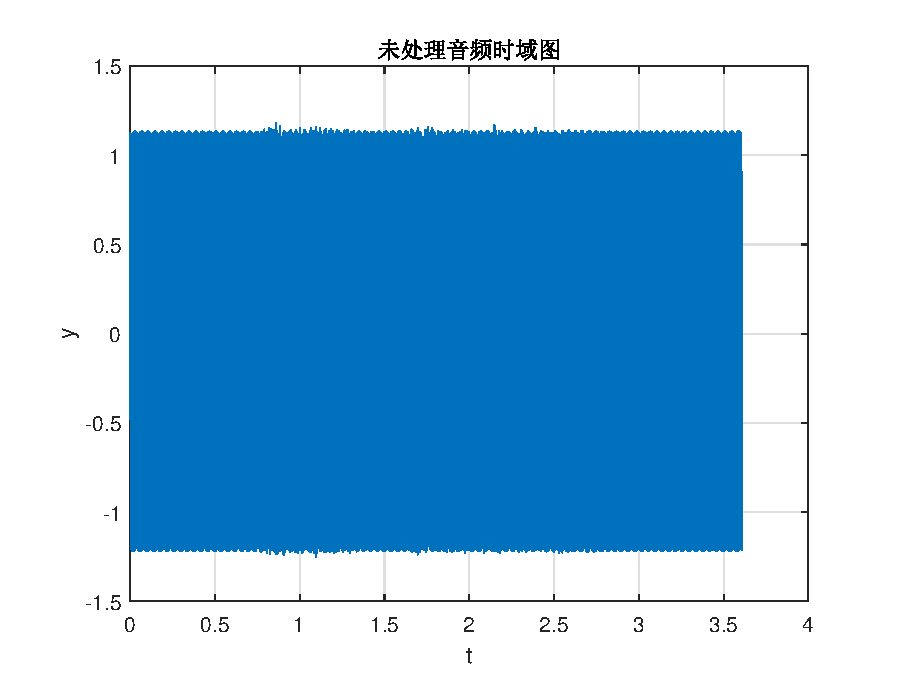
\includegraphics[width=8cm]{un-pict.eps}
    \caption{原音频信号时域图 }
\end{figure}
$\bullet$做音频信号频域图,并根据频域图像标记噪声频谱。\textit{此类噪声为单音噪声}\\\textit{单音噪声的消除首先考虑以某一幅度标准为限制,高于此幅度的进行滤除}
\begin{figure}[H]
    \centering
    \subcaptionbox{原音频信号频域图}{
        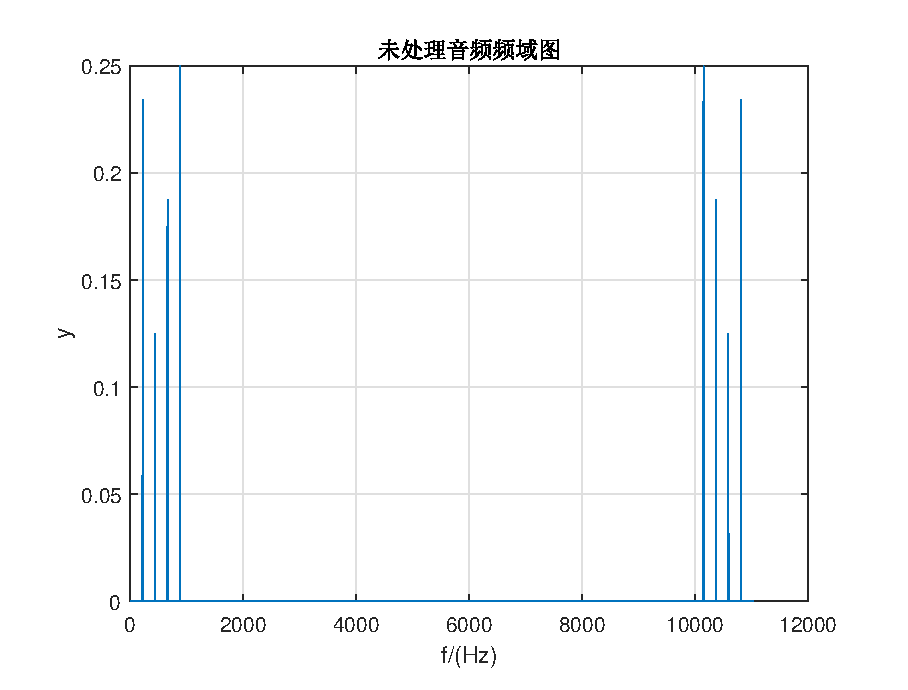
\includegraphics[width=11cm]{un-picf1.eps}	
    }
    \hfill 
    \subcaptionbox{原音频信号频域图-【标记噪声】}{
        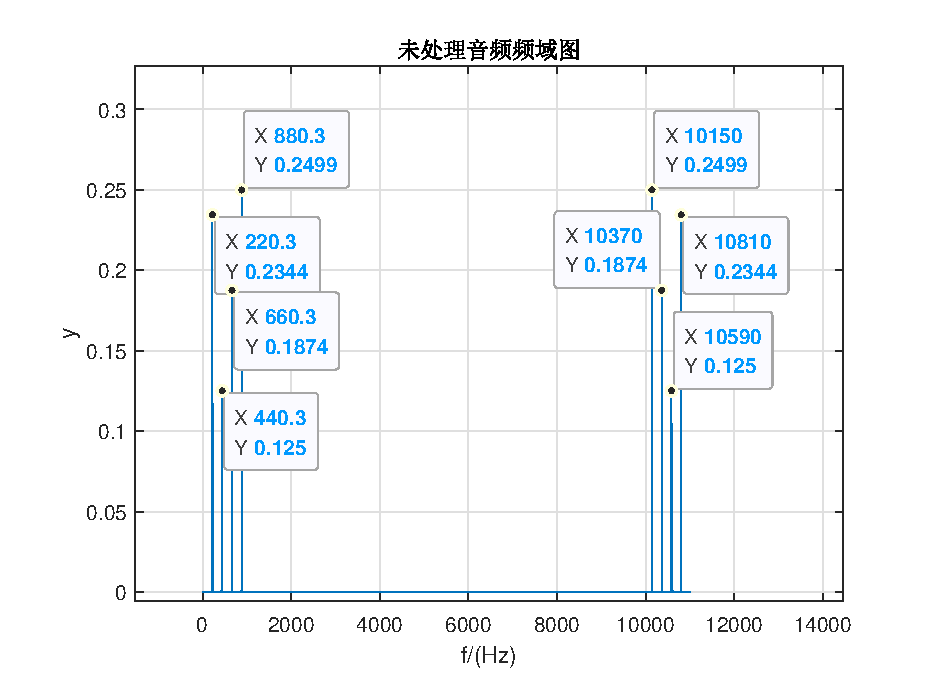
\includegraphics[width=11cm]{un-picf.eps}	
    }
    \caption{原音频信号频域图}
\end{figure}
\newpage
$\bullet$对音频信号进行初步处理。\textit{标记点y值:即为单音噪声滤除的幅度标准;标记点x值可判断出滤波器的上下限截止频率}\\
\indent 此时,已经可以消除绝大部分蜂鸣噪声,并辨析出该段音频在播放:\textit{‘这里是电子科技大学’}。

\begin{figure}[H]
    \centering
    \subcaptionbox{频域图}{
        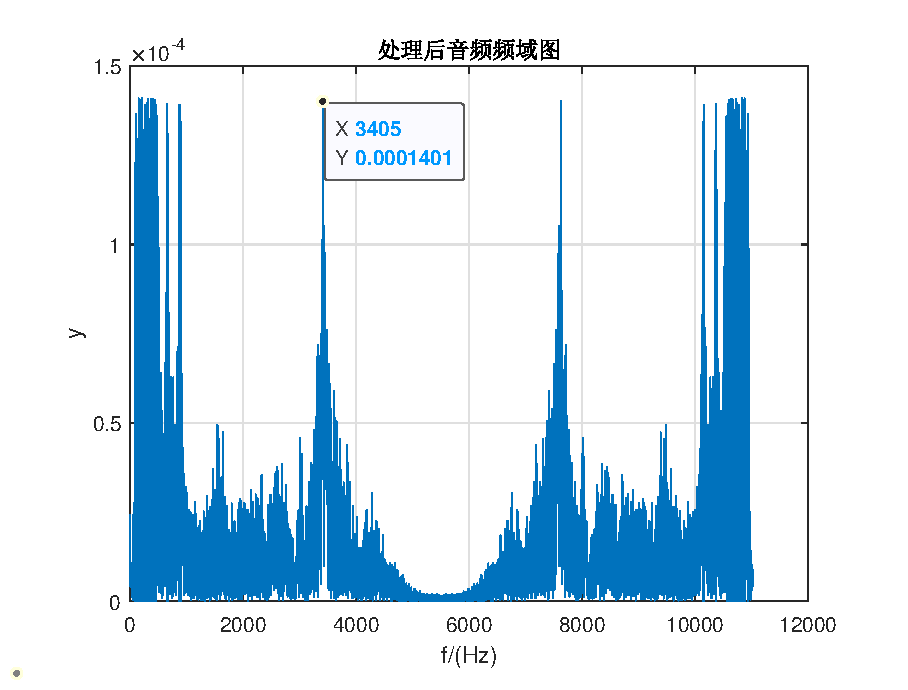
\includegraphics[width=11cm]{af-picf.eps}	
    }
    \hfill 
    \subcaptionbox{时域图}{
        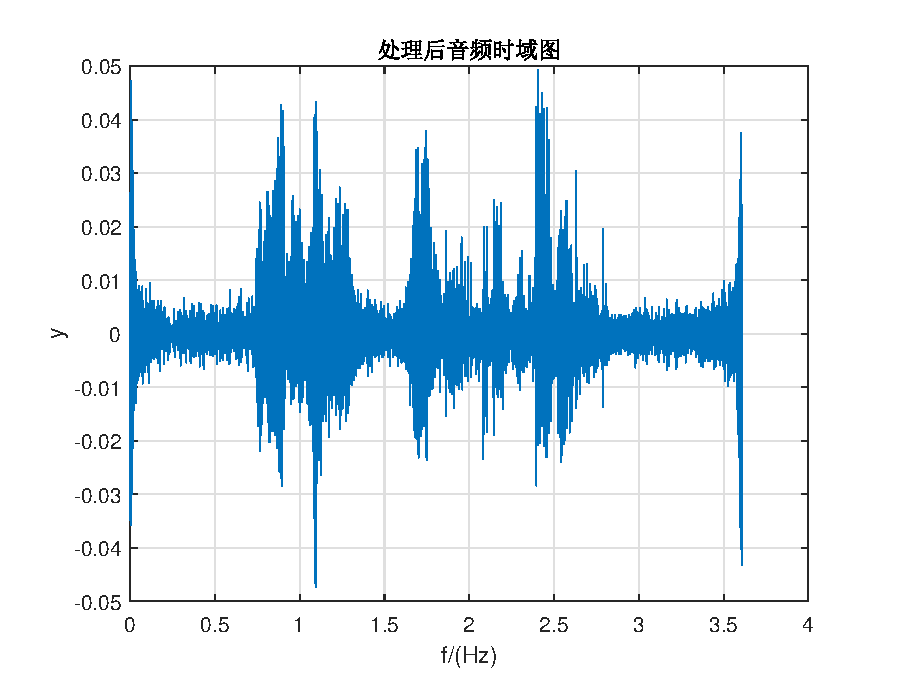
\includegraphics[width=11cm]{af-pict1.0.eps}	
    }
    \caption{一次处理后音频信号频域域图}
\end{figure}
\newpage
$\bullet$但是,第一步处理后听到处理音频仍伴随着持续低噪声,考虑使用带通滤波器直接去除双边频域信号.观测时域图也可发现,时域音频的‘毛刺’明显减少\\
\indent 此时持续低噪声明显消失,但此时人声听起来‘失真’,效果稍显不佳。\textit{(与初步处理音频相比更不像真人说话的效果,可以认为处理效果较为不佳)}

\begin{figure}[H]
    \centering
    \subcaptionbox{处理音频信号频域图}{
        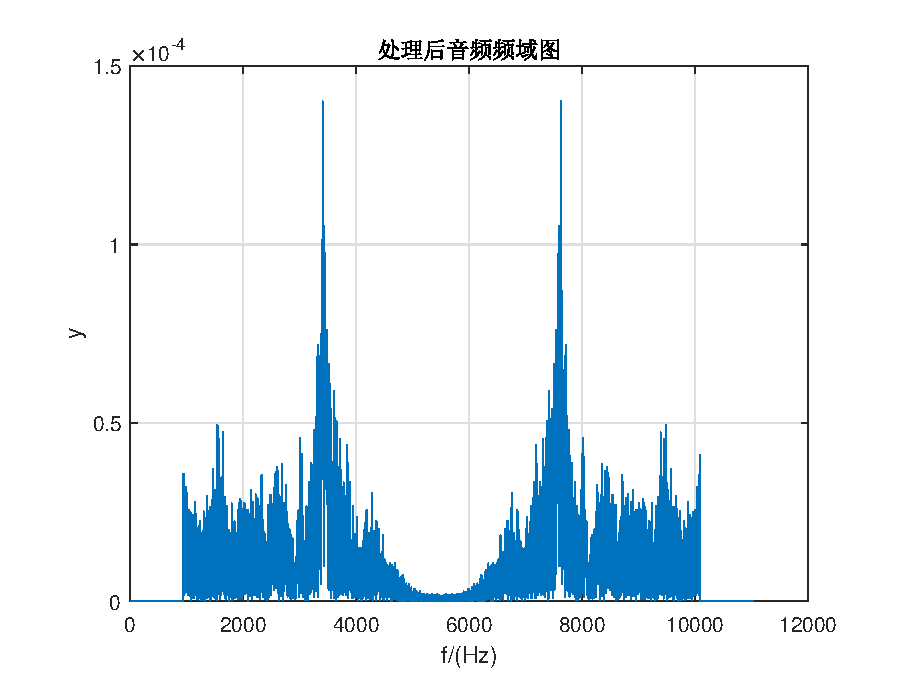
\includegraphics[width=11cm]{af-picf0.eps}	
    }
    \hfill 
    \subcaptionbox{处理音频信号时域图}{
        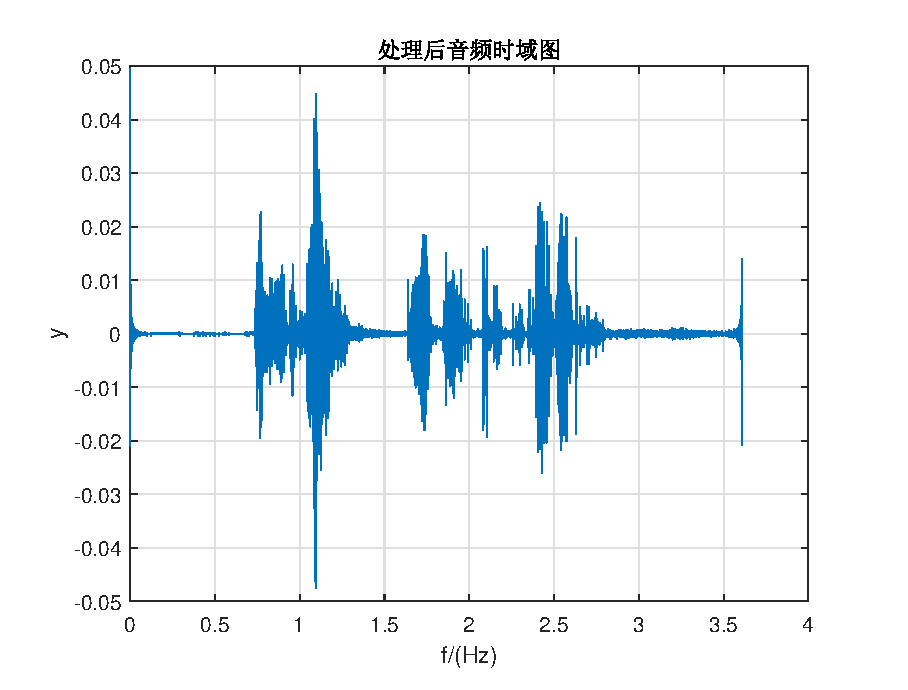
\includegraphics[width=11cm]{af-pict0.0.eps}	
    }
    \caption{全部滤波处理后音频信号频域域图}
\end{figure}
\newpage
$\bullet$ 人声听起来‘失真’,会不会是因为被滤去的双侧信号中仍含有部分音频信息呢?\\
\indent 于是,取双侧信号进行频域、时域分析,声音处理后仍可勉强辨识出,男声:‘这里是电子科技大学’。\\
\indent 不过,此时人声清晰度明显不足,且伴有较大噪声。但是仍可从此次变换中得到双侧\textbf{信号仍包含重要信息不应该被简单置零}的结论。\\
\begin{figure}[H]
    \centering
    \subcaptionbox{频域图}{
        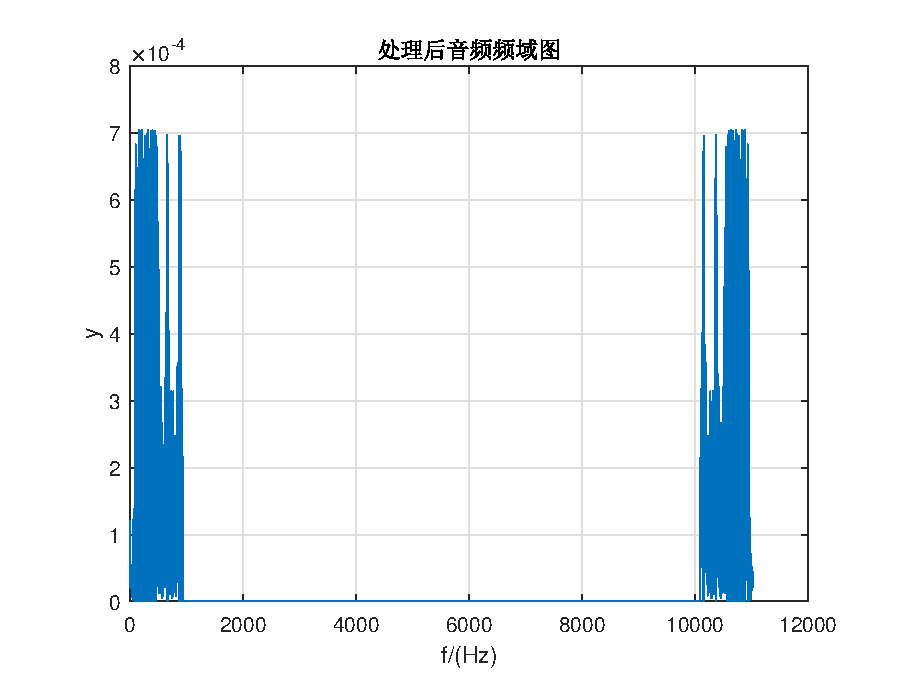
\includegraphics[width=10cm]{111.eps}	
    }
    \hfill 
    \subcaptionbox{时域图}{
        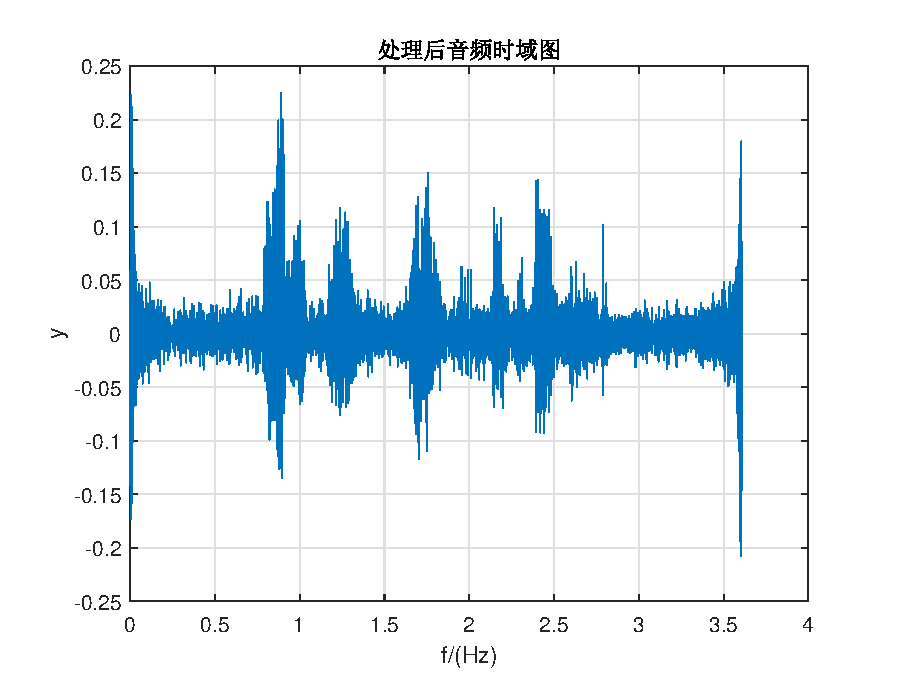
\includegraphics[width=10cm]{112.eps}	
    }
    \caption{双侧音频信号频域域图}
\end{figure}
$\bullet$ 那么可以知道双边频率信号的存在会带来与人声音量相近的持续低噪声,但是会使人声听起来‘更饱和’,于是考虑对双侧信号进行幅度调整减小噪音音量,而非直接滤除。\textit{【此部分噪声在单音噪声之间表现为没有个性的毛刺,故判断此段为宽频噪声,通过资料查询,可以使用幅度调制进行消减】}
\begin{figure}[H]
    \centering
    \
    \subcaptionbox{幅度调整为0.1倍-【频域】}{
        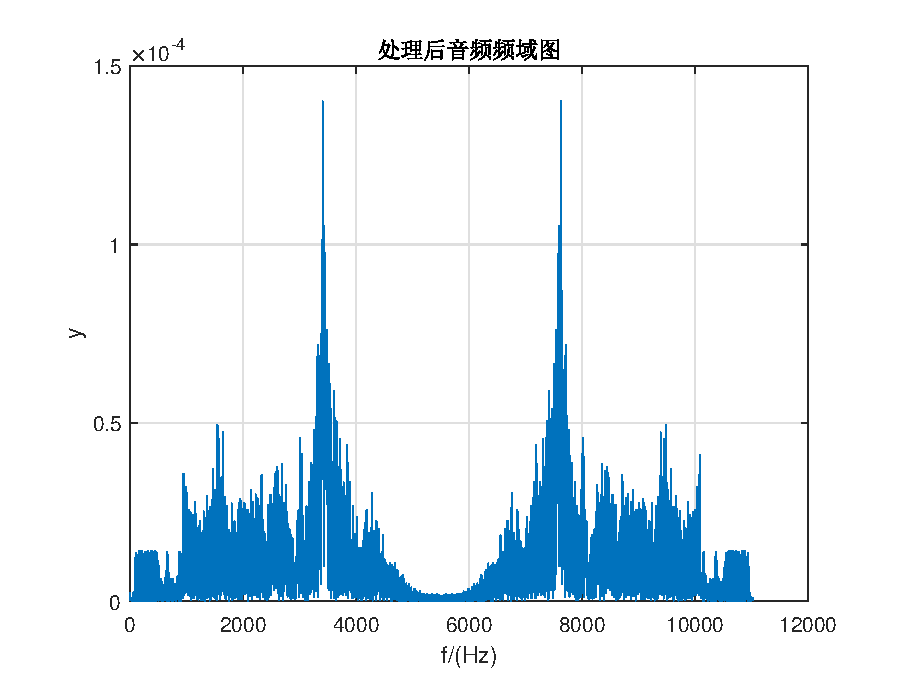
\includegraphics[width=7.2cm]{af-picf0.1.eps}	
    }
    \hfill 
    \subcaptionbox{幅度调整为0.1倍-【时域】}{
        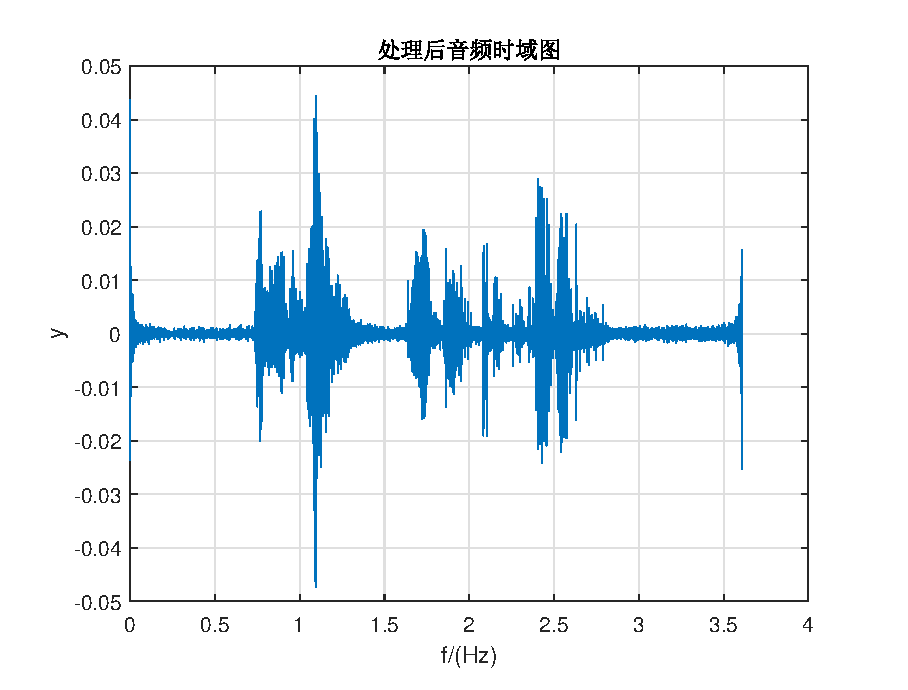
\includegraphics[width=7.2cm]{af-pict0.1.eps}	
    }
    \hfill 
    
    \subcaptionbox{幅度调整为0.5倍-【频域】}{
        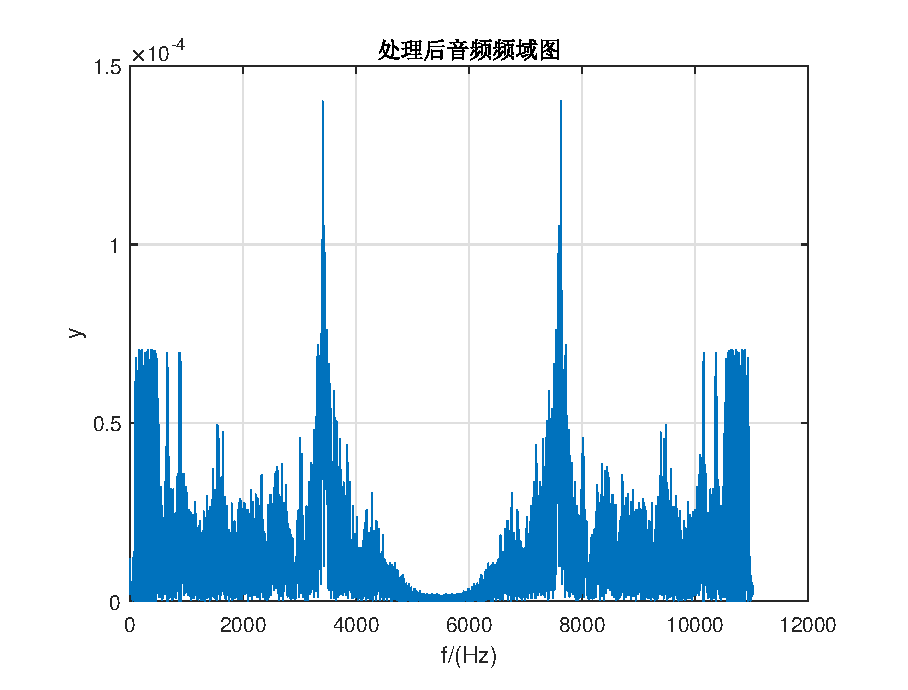
\includegraphics[width=7.2cm]{af-picf0.5.eps}	
    }
    \hfill 
    \subcaptionbox{幅度调整为0.5倍-【时域】}{
        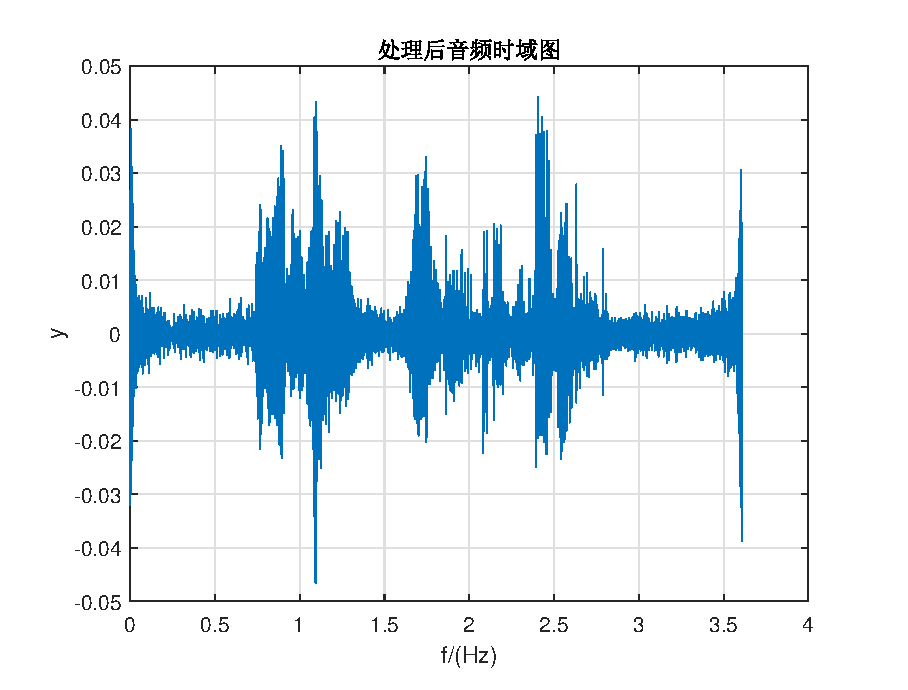
\includegraphics[width=7.2cm]{af-pict0.5.eps}	
    }
    \hfill 
    \subcaptionbox{幅度调整为0.8倍-【频域】}{
        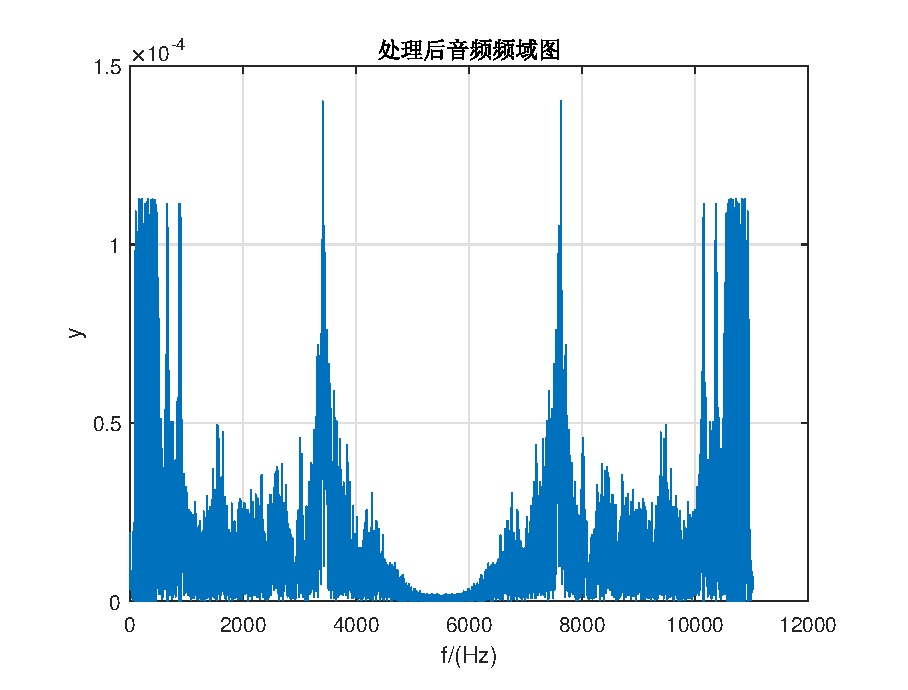
\includegraphics[width=7.2cm]{af-picf0.8.eps}	
    }
    \hfill 
    \subcaptionbox{幅度调整为0.8倍-【时域】}{
        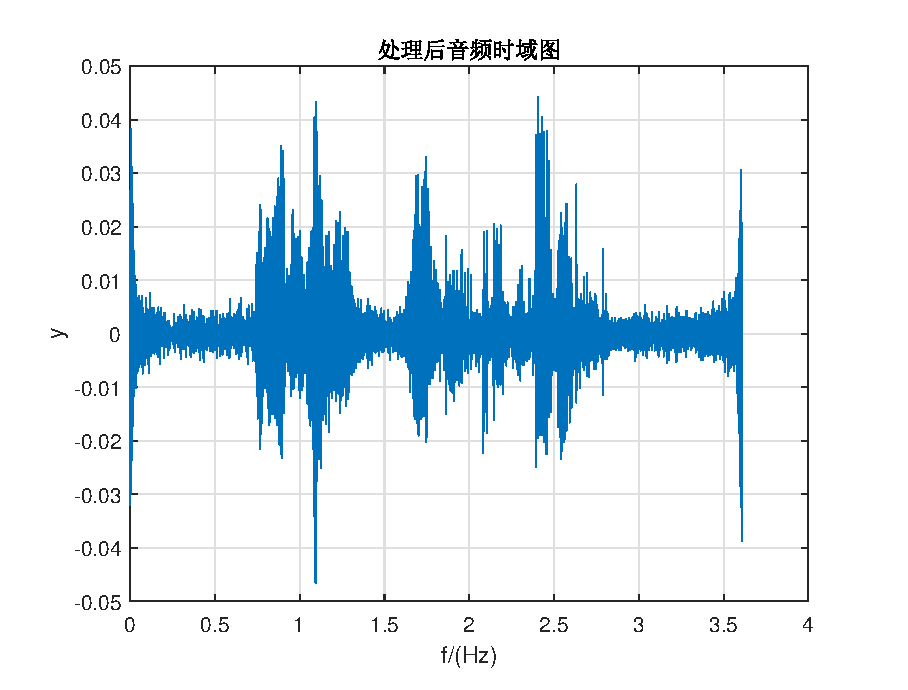
\includegraphics[width=7.2cm]{af-pict0.8.eps}	
    }
    \caption{多次测试-双侧信号幅度调制}
\end{figure} 
$\bullet$ 经过多次尝试,将幅度调整0.2倍时,可以保持人声的‘饱和’同时消减持续低噪声。此时,可认为目前去噪效果呈现为\textbf{最佳状态:可听出音频中男声‘这里是电子科技大学’,且音频噪声较小且人声饱满贴近真实声音}。
\begin{figure}[H]
    \centering
    \subcaptionbox{频域图}{
        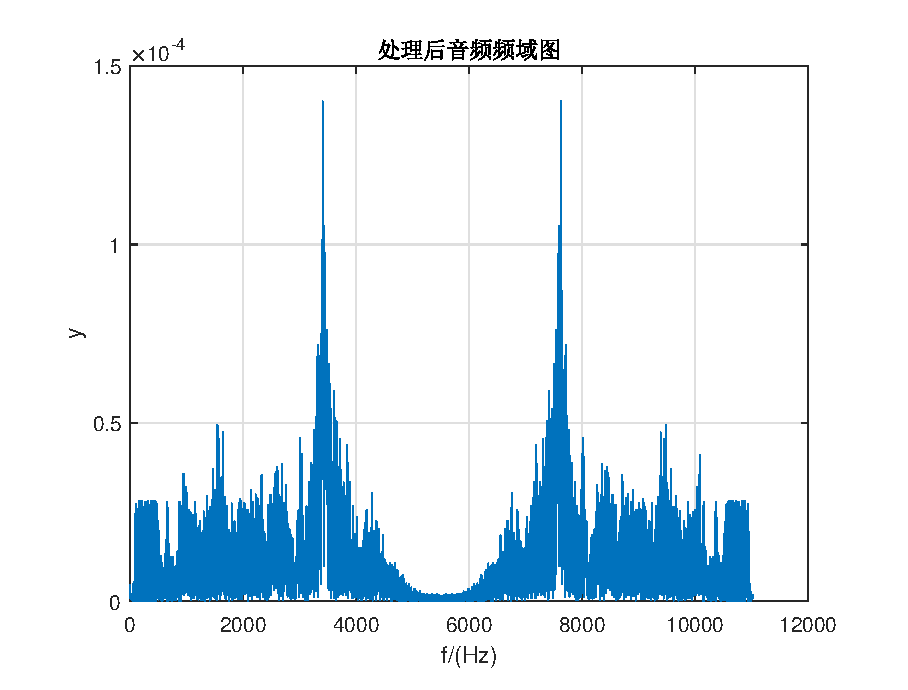
\includegraphics[width=11cm]{af-picf0.2.eps}	
    }
    \hfill 
    \subcaptionbox{时域图}{
        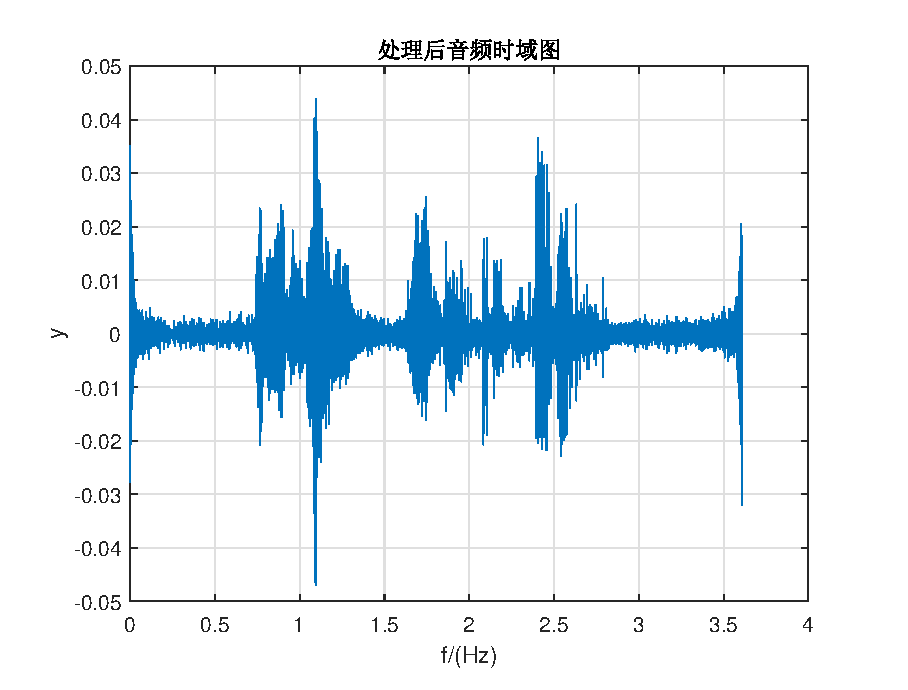
\includegraphics[width=11cm]{af-pict0.2.eps}	
    }
    \caption{最佳处理所得音频信号}
\end{figure}


%\section{设计名称}
去除干扰蜂鸣音
%\input{part2}
%\input{part3}
%\input{part4}
%\section{实验总结}
这次课程设计的主要原理是利用音频的幅频特性关系在频域将噪音信号去除,主要考察的是信号幅频特性以及滤波器的相关应用。\\
\indent 本设计的去除蜂鸣效果很好,且考虑到低频信号仍包含重要的人声要素,不可使用滤波器直接去除的问题。\textbf{可以将绝大部分的蜂鸣噪音全部去除,并且极高质量地保存了人声语言音频}\textit{【蜂鸣噪声绝大多数被消除且人声语言贴近真实声音、无明显‘失真’】},可以清晰地听到男声语音为:\textbf{“这里是电子科技大学”}。不过在音频开头、结尾仍有一小部分杂音没有去除,这或许是可以进一步改进的地方、但个人判断认为此声音可能是录音开启与结束的操作音直接存在于原始音频中,故而难以被滤除。\\
\indent 同时,本设计的功能相对更加开放,提供了许多可改变参数的参数,故此设计可以面向其他类似的音频使用,具有极大的扩展性。
%\input{strengths and weaknesses}
%


%

%\bibliographystyle{plain}
%\bibliography{ref}
%input{appendics}
%%%%%%%%%%%%%%%%%%%%%%%%%%%%%%
\end{document}
\end